\section{Proposed Method}

\subsection{Network}
The network used in the experiment is shown in Fig.\ref{fig:network_overall}.
The two main features of this method are a classification type output layer based on OCR methods and a camera-depth feature extractor based on the success in semantic segmentation.

%本手法では, OCRの手法を参考にしたclassification type output layerと, semantic segmentationでの成功を参考にしたRGB-D feature extractorの2つを大きな特徴とする。

\subsubsection{Camera-Depth Feature Extractor}
The feature extractor called SA-Gate used in this method\cite{SAGATE} is originally proposed by Chen et al. for semantic segmentation. SA-Gate's structure is shown in Fig.\ref{fig:sagate_overall}. As shown in Fig.\ref{fig:network_overall}, the feature extractor in this method uses the camera image and depth image as inputs and inputs the feature map obtained through the convolution layer to a special module called SA-Gate. The role of SA-Gate is to mitigate the influence of noise that inevitably gets mixed into the camera and depth image. In addition, SA-Gate has the role of recalibrating the two types of modalities from the camera image and the depth image and fusing the complementary information. The resulting feature map can be used as an input to the network for feature extraction that is more robust to noise. The parameter of the convolution layer of the feature extractor in this method is the pre-trained weight of ResNet\cite{he2015deep}, which enables efficient training and high classification ability.

%本手法で用いるfeature extractorは、semantic segmentationのためにChenらの研究で提案されたものを使用する。図AAAの通り、本手法のfeature extractorはcamera Imageとdepth imageの2つをinputとして、convolutional layerを通して得られたfeature mapをSA-Gateと言う特殊なモジュールへ入力する。このSA-Gateの役割はdepth画像にどうしても混入してしまうノイズ影響を緩和することに大きな効果がある。この他にも、SA-Gateにはcamera imageとdepth imageから来るtwo type modalitiesをrecalibrateしてcomplementary informationをfuseする役割を持つ、これによって得られたfeature mapをnetworkのinputとすることでよりノイズにロバストなfeature extractionを可能とする。本手法におけるfeature extractorのconvolutional layerのパラメータはResNetのpretrained weightを使用した。ResNetのpretrained weightを使用することで効率的な学習と高い識別能力を獲得することができた。

\begin{figure}[thpb]
\centering
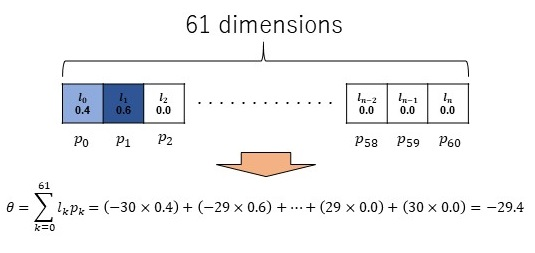
\includegraphics[scale=0.5]{./figure/2_method/classification_layer.jpg}
\caption{Classification Type Output Layer}
\label{fig:classification_layer}
\end{figure}

\subsubsection{Classification Type Output Layer}
In a previous study, we achieved high accuracy in attitude estimation by introducing a classification type network\cite{9708864}, which has shown high performance in the field of OCR\cite{kuzushiji_dl}, to the attitude estimation task. Handwritten characters vary greatly in form depending on the writer and the period in which they were written. However, the network equipped with a classification type output layer shown in Fig.\ref{fig:classification_layer} has acquired a high recognition ability. In addition, the landscape image captured by the camera differs greatly depending on the location, even at the same angle of orientation. In a previous study, we found commonalities between two different types of tasks in this location and introduced a classification type network for the attitude estimation task. The results showed that the classification type network had the best accuracy in terms of attitude estimation accuracy compared to the existing numerical regression type network.

The output layer of the classification type is limited in the range of angles it handles, unlike the numerical regression type, but within that range, it can perform high recognition ability. This is because cross-entropy loss is introduced during training. Cross-entropy loss provides the benefits of the theory of maximum likelihood estimation that enables efficient Bayesian inference by specifying a conjugate prior.

The experiments in this paper deal with angles from -30 to +30 degrees. Since this method is designed to be mounted on a robot in Fig.\ref{fig:CCV}, it does not have the same problems as drones even if the angles to be handled are limited. In this paper, the classification type output layer has 61 dimensions. This is the result of assigning the corresponding index to each angle, such as index 0 for -30 degrees, index 1 for -29 degrees, and so on. Each index expresses the probability of an angle within the range of 0 to 1. For example, if an angle of -29.40[deg] is to be represented as the correct answer label in the class identification network, the 0th index assigned as -30.0 degrees is assigned a value of 0.40, and the 1st index assigned as -29.0 degrees is assigned a value of 0.60. In this way, the output layer of the class identification neural network, which can only represent values from 0.0 to 1.0, can also represent values from -30.0 to 30.0.

%以前の研究で我々はOCRの分野で高い性能を発揮しているclassification type networkをattitude estimationタスクに導入することで高いattitude estimation accuracyを達成した。手書きの文字は書く人や書かれた時代によって字の形は大きく異る。しかし、classification type output layerを備えたネットワークで学習することで高い識別能力を獲得している。また、カメラ画像についても同じ姿勢角であっても場所によって撮影される風景画像は大きく異る。以前の研究において、我々はこの箇所に2つの異なる種類のタスク間での共通性を見出し、attitude estimation taskにclassification type networkを導入した。この結果、classification type networkのattitude estimation accurcyは既存のnumerical regression type networkと比較して最も良い精度であった。

%classification typeの出力層は扱う角度の範囲はnumerical regression typeとは異なり限定されるが、その範囲内では高い識別能力を持っている。これは学習時にcross entropy lossを導入しているためである。クロスエントロピー損失は、共役事前分布を指定することで効率的なベイズ推定を可能にするという最尤推定の理論の利点を提供する。

%本論文での実験では、-30度から+30度までの角度を扱う。本手法はAAAAAのようなロボットにおいて搭載することを前提としているため、扱う角度が限定されてもドローンのような問題は発生しない。本論文においてclassification type output layerは61次元を取る。これは-30度にはインデックス0、-29度にはインデックス1といったように角度に応じて対応するインデックスを割り振っていった結果である。それぞれのインデックスは0から1までの範囲内で角度の確率を表現する。例えば-29.55[deg]という角度をクラス識別ネットワークの正解ラベルとして表現したい場合、-30.0度として割り振られた0番目のインデックスには0.55、-29.0度として割り振られた1番目のインデックスには0.45の値をそれぞれ割り振る。このようにすることで0.0から1.0までしか表現できないクラス識別ニューラルネットワークの出力層でも-30.0から30.0までの値を表現することができる。


\subsection{Random Window Method for Input Image}\label{sec:random_window}
In this method, the center position of the input image is randomly selected, and inference is performed using multiple images cropped from the center of the image, which is also used in OCR methods\cite{OCR_paper}. The probability distribution obtained by inference using multiple images clipped at a randomly selected center position is different each time. These are averaged to compensate for the inference error. Such clipped images are used not only for inference but also for generating training data.

%本手法ではOCRの手法でも用いられている、入力画像に対して中心位置をランダムに選び、そこを中心に切り抜かれた画像を複数枚用いて推論を行う。中心位置をランダムに選択して切り抜いた複数枚の画像を用いて推論すると得られる確率分布は毎回異なるものが得られる。これらを平均することで推論の誤差をcompensateしている。このような画像の切り抜きは推論のときだけでなく、学習用データの生成時にも使用される。

\begin{figure}[thpb]
\centering
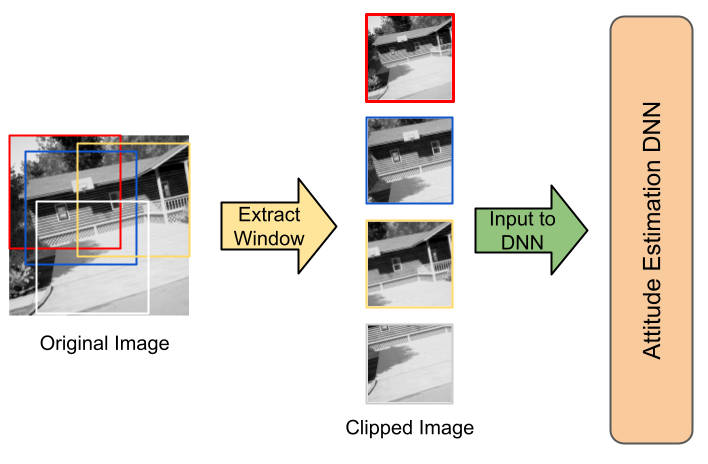
\includegraphics[scale=0.4]{./figure/2_method/RandomWindow_2.png}
\caption{Extraction Windows from Original Camera Image.}
\label{fig:extract_windows}
\end{figure}